\documentclass[twoside]{book}

% Packages required by doxygen
\usepackage{fixltx2e}
\usepackage{calc}
\usepackage{doxygen}
\usepackage[export]{adjustbox} % also loads graphicx
\usepackage{graphicx}
\usepackage[utf8]{inputenc}
\usepackage{makeidx}
\usepackage{multicol}
\usepackage{multirow}
\PassOptionsToPackage{warn}{textcomp}
\usepackage{textcomp}
\usepackage[nointegrals]{wasysym}
\usepackage[table]{xcolor}

% Font selection
\usepackage[T1]{fontenc}
\usepackage[scaled=.90]{helvet}
\usepackage{courier}
\usepackage{amssymb}
\usepackage{sectsty}
\renewcommand{\familydefault}{\sfdefault}
\allsectionsfont{%
  \fontseries{bc}\selectfont%
  \color{darkgray}%
}
\renewcommand{\DoxyLabelFont}{%
  \fontseries{bc}\selectfont%
  \color{darkgray}%
}
\newcommand{\+}{\discretionary{\mbox{\scriptsize$\hookleftarrow$}}{}{}}

% Page & text layout
\usepackage{geometry}
\geometry{%
  a4paper,%
  top=2.5cm,%
  bottom=2.5cm,%
  left=2.5cm,%
  right=2.5cm%
}
\tolerance=750
\hfuzz=15pt
\hbadness=750
\setlength{\emergencystretch}{15pt}
\setlength{\parindent}{0cm}
\setlength{\parskip}{0.2cm}
\makeatletter
\renewcommand{\paragraph}{%
  \@startsection{paragraph}{4}{0ex}{-1.0ex}{1.0ex}{%
    \normalfont\normalsize\bfseries\SS@parafont%
  }%
}
\renewcommand{\subparagraph}{%
  \@startsection{subparagraph}{5}{0ex}{-1.0ex}{1.0ex}{%
    \normalfont\normalsize\bfseries\SS@subparafont%
  }%
}
\makeatother

% Headers & footers
\usepackage{fancyhdr}
\pagestyle{fancyplain}
\fancyhead[LE]{\fancyplain{}{\bfseries\thepage}}
\fancyhead[CE]{\fancyplain{}{}}
\fancyhead[RE]{\fancyplain{}{\bfseries\leftmark}}
\fancyhead[LO]{\fancyplain{}{\bfseries\rightmark}}
\fancyhead[CO]{\fancyplain{}{}}
\fancyhead[RO]{\fancyplain{}{\bfseries\thepage}}
\fancyfoot[LE]{\fancyplain{}{}}
\fancyfoot[CE]{\fancyplain{}{}}
\fancyfoot[RE]{\fancyplain{}{\bfseries\scriptsize Generated on Tue Jun 16 2015 00\+:20\+:50 for Projeto Disk by Doxygen }}
\fancyfoot[LO]{\fancyplain{}{\bfseries\scriptsize Generated on Tue Jun 16 2015 00\+:20\+:50 for Projeto Disk by Doxygen }}
\fancyfoot[CO]{\fancyplain{}{}}
\fancyfoot[RO]{\fancyplain{}{}}
\renewcommand{\footrulewidth}{0.4pt}
\renewcommand{\chaptermark}[1]{%
  \markboth{#1}{}%
}
\renewcommand{\sectionmark}[1]{%
  \markright{\thesection\ #1}%
}

% Indices & bibliography
\usepackage{natbib}
\usepackage[titles]{tocloft}
\setcounter{tocdepth}{3}
\setcounter{secnumdepth}{5}
\makeindex

% Hyperlinks (required, but should be loaded last)
\usepackage{ifpdf}
\ifpdf
  \usepackage[pdftex,pagebackref=true]{hyperref}
\else
  \usepackage[ps2pdf,pagebackref=true]{hyperref}
\fi
\hypersetup{%
  colorlinks=true,%
  linkcolor=blue,%
  citecolor=blue,%
  unicode%
}

% Custom commands
\newcommand{\clearemptydoublepage}{%
  \newpage{\pagestyle{empty}\cleardoublepage}%
}


%===== C O N T E N T S =====

\begin{document}

% Titlepage & ToC
\hypersetup{pageanchor=false,
             bookmarks=true,
             bookmarksnumbered=true,
             pdfencoding=unicode
            }
\pagenumbering{roman}
\begin{titlepage}
\vspace*{7cm}
\begin{center}%
{\Large Projeto Disk }\\
\vspace*{1cm}
{\large Generated by Doxygen 1.8.9.1}\\
\vspace*{0.5cm}
{\small Tue Jun 16 2015 00:20:50}\\
\end{center}
\end{titlepage}
\clearemptydoublepage
\tableofcontents
\clearemptydoublepage
\pagenumbering{arabic}
\hypersetup{pageanchor=true}

%--- Begin generated contents ---
\chapter{R\+E\+A\+D\+M\+E}
\label{md_README}
\hypertarget{md_README}{}
$<$$<$$<$$<$$<$$<$$<$ H\+E\+A\+D \section*{\#\#\+Trabalho da Terceira Unidade E\+D\+B1/\+L\+P1\#\#}

Autores\+: Ana Clara (github.\+com/claranobre) e Rai Vitor (github.\+com/rai-\/vitor)

\section*{$\ast$$\ast$ P\+R\+O\+J\+E\+T\+O G\+E\+R\+E\+N\+C\+I\+A\+D\+O\+R D\+E D\+I\+S\+C\+O $\ast$$\ast$}

\subparagraph*{O projeto \char`\"{}\+Gerenciador de Disco\char`\"{} foi criado para pôr em prático os conceitos de Estrutura de Dados visto em sala de aula, manipulação de arquivo e operações com lista, nele é possível um usuário criar um arquivo e executar operações no disco criado}

\section*{$\ast$$\ast$\+Execução$\ast$$\ast$}

\subparagraph*{O usuário deve entrar no diretório do projeto \char`\"{}project\+\_\+disk\char`\"{} pelo terminal Linux ou Terminal simulador(\+C\+Y\+G\+W\+I\+N) do Windows}

\subparagraph*{Estando dentro do diretório o usuário deve entrar no diretório criado pela biblioteca gráfica utilizada para execução do projeto (Qt creator)\+: build-\/\+Gerenciador\+De\+Disco-\/\+Desktop\+\_\+\+Qt\+\_\+5\+\_\+4\+\_\+1\+\_\+\+G\+C\+C\+\_\+64bit-\/\+Debug }

\subparagraph*{Estando dentro do diretório o usuário deve escrever o comando \char`\"{}make\char`\"{}}

\subparagraph*{Ao terminar o comando será criado o objeto executável denominado \char`\"{}\+Gerenciador\+De\+Disco\char`\"{}}

\subparagraph*{Uma vez dentro do diretório o usuário só precisa clicar no executável ./\+Gerenciador\+De\+Disco}

\subparagraph*{Ao terminar de manipular o Gerenciador o usuário só precisa fechá-\/lo no botão de sair do software e todos os dados armazenados serão perdidos}

\section*{$\ast$$\ast$\+Verificação de Vazamento de Memória$\ast$$\ast$ }

\subparagraph*{Para verificarmos se o nosso algoritmo está com vazamento de memória de dados, utilizamos a ferramenta Valgrind para teste}

\subparagraph*{O usuário após compilar e criar o objeto deve escrever no Terminal\+:}

{\itshape valgrind --leak-\/check=full ./\+Gerenciador\+De\+Disco}

\section*{$\ast$$\ast$\+Documentação$\ast$$\ast$}

\section*{Foi utilizada a ferramenta Doxygen para auxiliar na documentação da execução desse projeto, para o usuário visualizar é necessário entrar no diretório \char`\"{}html\char`\"{} e acessar o arquivo index.\+html, logo a documentação será aberta em modo offline em seu navegador padrão}

\section*{Simulador de \hyperlink{classDisco}{Disco}}

\subsubsection*{Nome e Matrícula}

Ana Clara Nobre Mendes -\/ 2013002964 Raí Vitor Morais da Silva -\/ 2014000900

\subsubsection*{Como Executar o programa}

cd Gerenciador\+De\+Disco

./\+Gerenciador\+De\+Disco

\subsubsection*{Makefile}

Gerenciador\+De\+Disco/\+Makefile

\begin{quote}
\begin{quote}
\begin{quote}
\begin{quote}
\begin{quote}
\begin{quote}
\begin{quote}
68db918b62a0482479cdb64b5e981ab6a9dba924\end{quote}
\end{quote}
\end{quote}
\end{quote}
\end{quote}
\end{quote}
\end{quote}

\chapter{Hierarchical Index}
\section{Class Hierarchy}
This inheritance list is sorted roughly, but not completely, alphabetically\+:\begin{DoxyCompactList}
\item \contentsline{section}{Disco}{\pageref{classDisco}}{}
\item \contentsline{section}{File}{\pageref{classFile}}{}
\item \contentsline{section}{Lista$<$ type $>$}{\pageref{classLista}}{}
\item \contentsline{section}{Lista$<$ File $\ast$ $>$}{\pageref{classLista}}{}
\item \contentsline{section}{Lista$<$ Setor $\ast$ $>$}{\pageref{classLista}}{}
\item \contentsline{section}{Lista$<$ type $>$\+:\+:node}{\pageref{structLista_1_1node}}{}
\item Q\+Dialog\begin{DoxyCompactList}
\item \contentsline{section}{Dialog}{\pageref{classDialog}}{}
\end{DoxyCompactList}
\item Q\+Main\+Window\begin{DoxyCompactList}
\item \contentsline{section}{Main\+Window}{\pageref{classMainWindow}}{}
\end{DoxyCompactList}
\item \contentsline{section}{qt\+\_\+meta\+\_\+stringdata\+\_\+\+Dialog\+\_\+t}{\pageref{structqt__meta__stringdata__Dialog__t}}{}
\item \contentsline{section}{qt\+\_\+meta\+\_\+stringdata\+\_\+\+Main\+Window\+\_\+t}{\pageref{structqt__meta__stringdata__MainWindow__t}}{}
\item \contentsline{section}{Setor}{\pageref{classSetor}}{}
\item \contentsline{section}{Ui\+\_\+\+Dialog}{\pageref{classUi__Dialog}}{}
\begin{DoxyCompactList}
\item \contentsline{section}{Ui\+:\+:Dialog}{\pageref{classUi_1_1Dialog}}{}
\item \contentsline{section}{Ui\+:\+:Dialog}{\pageref{classUi_1_1Dialog}}{}
\end{DoxyCompactList}
\item \contentsline{section}{Ui\+\_\+\+Main\+Window}{\pageref{classUi__MainWindow}}{}
\begin{DoxyCompactList}
\item \contentsline{section}{Ui\+:\+:Main\+Window}{\pageref{classUi_1_1MainWindow}}{}
\item \contentsline{section}{Ui\+:\+:Main\+Window}{\pageref{classUi_1_1MainWindow}}{}
\end{DoxyCompactList}
\end{DoxyCompactList}

\chapter{Class Index}
\section{Class List}
Here are the classes, structs, unions and interfaces with brief descriptions\+:\begin{DoxyCompactList}
\item\contentsline{section}{\hyperlink{classUi_1_1Dialog}{Ui\+::\+Dialog} }{\pageref{classUi_1_1Dialog}}{}
\item\contentsline{section}{\hyperlink{classDialog}{Dialog} \\*Classe da primeira tela do sistema. Pega os valores do usuário para realmente iniciar o sistema }{\pageref{classDialog}}{}
\item\contentsline{section}{\hyperlink{classDisco}{Disco} \\*Classe que controla todos as funções do disco }{\pageref{classDisco}}{}
\item\contentsline{section}{\hyperlink{classFile}{File} \\*Classe que guarda os arquivos salvos }{\pageref{classFile}}{}
\item\contentsline{section}{\hyperlink{classLista}{Lista$<$ type $>$} \\*Classe genérica de \hyperlink{classLista}{Lista} encadeadas, pode se comportar como \hyperlink{classLista}{Lista} simples, fila ou pilha }{\pageref{classLista}}{}
\item\contentsline{section}{\hyperlink{classUi_1_1MainWindow}{Ui\+::\+Main\+Window} }{\pageref{classUi_1_1MainWindow}}{}
\item\contentsline{section}{\hyperlink{classMainWindow}{Main\+Window} }{\pageref{classMainWindow}}{}
\item\contentsline{section}{\hyperlink{structLista_1_1node}{Lista$<$ type $>$\+::node} }{\pageref{structLista_1_1node}}{}
\item\contentsline{section}{\hyperlink{structqt__meta__stringdata__Dialog__t}{qt\+\_\+meta\+\_\+stringdata\+\_\+\+Dialog\+\_\+t} }{\pageref{structqt__meta__stringdata__Dialog__t}}{}
\item\contentsline{section}{\hyperlink{structqt__meta__stringdata__MainWindow__t}{qt\+\_\+meta\+\_\+stringdata\+\_\+\+Main\+Window\+\_\+t} }{\pageref{structqt__meta__stringdata__MainWindow__t}}{}
\item\contentsline{section}{\hyperlink{classSetor}{Setor} }{\pageref{classSetor}}{}
\item\contentsline{section}{\hyperlink{classUi__Dialog}{Ui\+\_\+\+Dialog} }{\pageref{classUi__Dialog}}{}
\item\contentsline{section}{\hyperlink{classUi__MainWindow}{Ui\+\_\+\+Main\+Window} }{\pageref{classUi__MainWindow}}{}
\end{DoxyCompactList}

\chapter{Class Documentation}
\hypertarget{classDialog}{\section{Dialog Class Reference}
\label{classDialog}\index{Dialog@{Dialog}}
}


Classe da primeira tela do sistema. Pega os valores do usuário para realmente iniciar o sistema.  




{\ttfamily \#include $<$dialog.\+h$>$}

Inheritance diagram for Dialog\+:\begin{figure}[H]
\begin{center}
\leavevmode
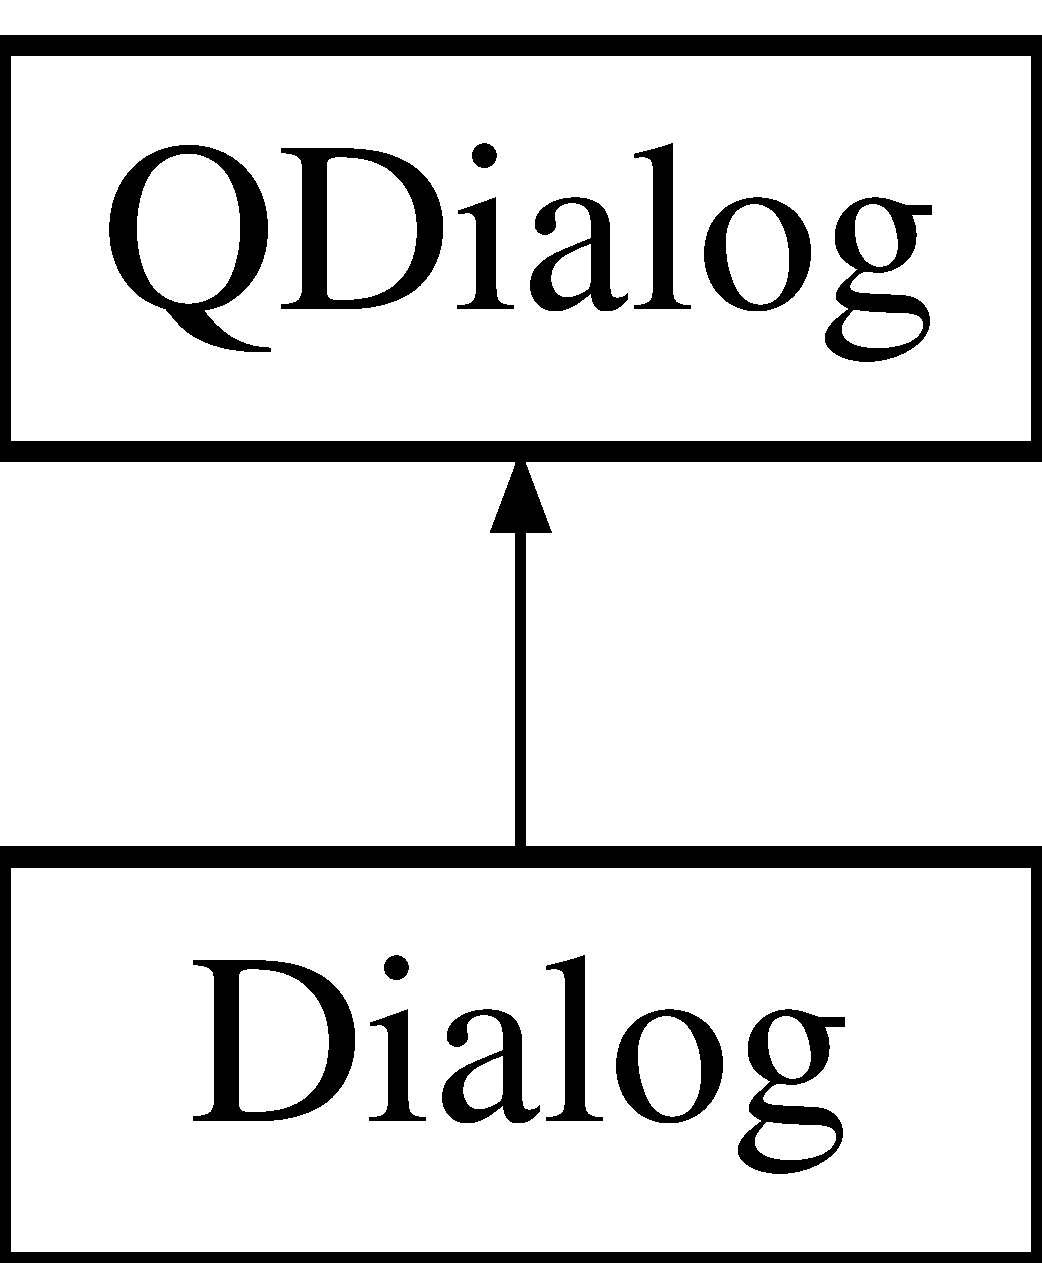
\includegraphics[height=2.000000cm]{classDialog}
\end{center}
\end{figure}
\subsection*{Public Member Functions}
\begin{DoxyCompactItemize}
\item 
\hypertarget{classDialog_acfa2063f9f962d394c6a645b6e7e08d8}{{\bfseries Dialog} (Q\+Widget $\ast$parent=0)}\label{classDialog_acfa2063f9f962d394c6a645b6e7e08d8}

\item 
int \hyperlink{classDialog_a6b0119c5bf8caa17599f5886dbbfc785}{get\+Quant\+Setor} () const 
\item 
int \hyperlink{classDialog_ac632d4306f67630cc30a1706323819bb}{get\+Tam\+Disco} () const 
\item 
int \hyperlink{classDialog_a7b5648b3e00170bd86f875de20f17eda}{get\+Tam\+Setor} () const 
\end{DoxyCompactItemize}


\subsection{Detailed Description}
Classe da primeira tela do sistema. Pega os valores do usuário para realmente iniciar o sistema. 

\subsection{Member Function Documentation}
\hypertarget{classDialog_a6b0119c5bf8caa17599f5886dbbfc785}{\index{Dialog@{Dialog}!get\+Quant\+Setor@{get\+Quant\+Setor}}
\index{get\+Quant\+Setor@{get\+Quant\+Setor}!Dialog@{Dialog}}
\subsubsection[{get\+Quant\+Setor}]{\setlength{\rightskip}{0pt plus 5cm}int Dialog\+::get\+Quant\+Setor (
\begin{DoxyParamCaption}
{}
\end{DoxyParamCaption}
) const}}\label{classDialog_a6b0119c5bf8caa17599f5886dbbfc785}
Retorna a quantidade de setores \begin{DoxyReturn}{Returns}
retorna a quantidade de setores 
\end{DoxyReturn}
\hypertarget{classDialog_ac632d4306f67630cc30a1706323819bb}{\index{Dialog@{Dialog}!get\+Tam\+Disco@{get\+Tam\+Disco}}
\index{get\+Tam\+Disco@{get\+Tam\+Disco}!Dialog@{Dialog}}
\subsubsection[{get\+Tam\+Disco}]{\setlength{\rightskip}{0pt plus 5cm}int Dialog\+::get\+Tam\+Disco (
\begin{DoxyParamCaption}
{}
\end{DoxyParamCaption}
) const}}\label{classDialog_ac632d4306f67630cc30a1706323819bb}
Retorna o tamanho do disco \begin{DoxyReturn}{Returns}
retorna o tamanho do disco 
\end{DoxyReturn}
\hypertarget{classDialog_a7b5648b3e00170bd86f875de20f17eda}{\index{Dialog@{Dialog}!get\+Tam\+Setor@{get\+Tam\+Setor}}
\index{get\+Tam\+Setor@{get\+Tam\+Setor}!Dialog@{Dialog}}
\subsubsection[{get\+Tam\+Setor}]{\setlength{\rightskip}{0pt plus 5cm}int Dialog\+::get\+Tam\+Setor (
\begin{DoxyParamCaption}
{}
\end{DoxyParamCaption}
) const}}\label{classDialog_a7b5648b3e00170bd86f875de20f17eda}
Retorna o tamanho do setor \begin{DoxyReturn}{Returns}
retorna o tamanho do setor 
\end{DoxyReturn}


The documentation for this class was generated from the following files\+:\begin{DoxyCompactItemize}
\item 
Gerenciador\+De\+Disco/dialog.\+h\item 
Gerenciador\+De\+Disco/dialog.\+cpp\end{DoxyCompactItemize}

\hypertarget{classUi_1_1Dialog}{}\section{Ui\+:\+:Dialog Class Reference}
\label{classUi_1_1Dialog}\index{Ui\+::\+Dialog@{Ui\+::\+Dialog}}
Inheritance diagram for Ui\+:\+:Dialog\+:\begin{figure}[H]
\begin{center}
\leavevmode
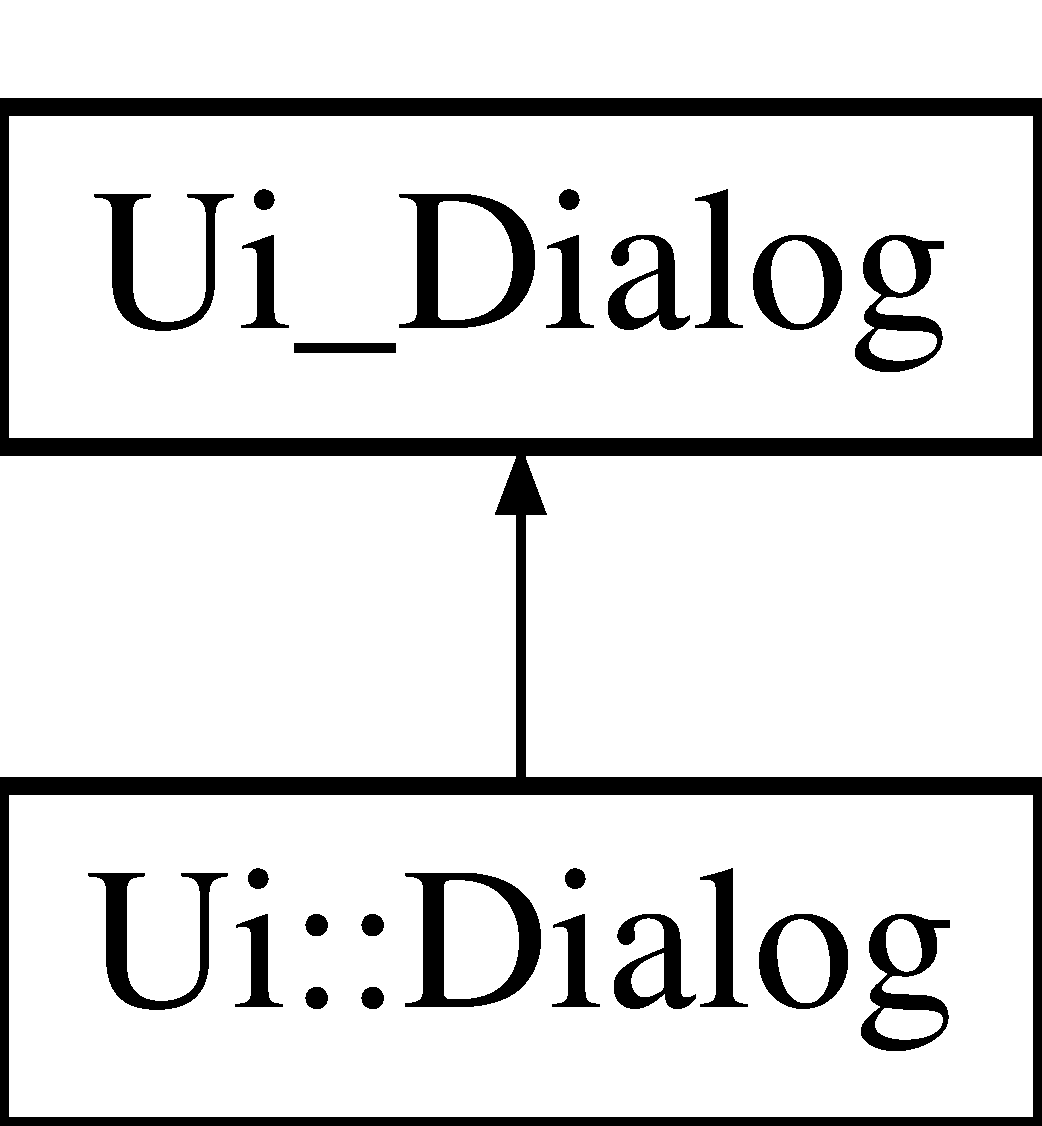
\includegraphics[height=2.000000cm]{classUi_1_1Dialog}
\end{center}
\end{figure}
\subsection*{Additional Inherited Members}


The documentation for this class was generated from the following file\+:\begin{DoxyCompactItemize}
\item 
build-\/\+Gerenciador\+De\+Disco-\/\+Desktop\+\_\+\+Qt\+\_\+5\+\_\+4\+\_\+1\+\_\+\+G\+C\+C\+\_\+64bit-\/\+Debug/ui\+\_\+dialog.\+h\end{DoxyCompactItemize}

\hypertarget{classDisco}{}\section{Disco Class Reference}
\label{classDisco}\index{Disco@{Disco}}


Classe que controla todos as funções do disco.  




{\ttfamily \#include $<$disco.\+h$>$}

\subsection*{Public Member Functions}
\begin{DoxyCompactItemize}
\item 
\hyperlink{classDisco_a8f87658574d2528cb32b4c975716fa38}{Disco} (int quant\+Setores, int tam\+Setores, int tam\+Disco)
\item 
\hyperlink{classDisco_a9e8131123ed8969c7608ce877c765029}{$\sim$\+Disco} ()
\item 
int \hyperlink{classDisco_af09da728510fdb43fa68430e743ab7c4}{Salvar} (const char $\ast$str\+Value, int tam\+Value, string str\+Nome)
\item 
int \hyperlink{classDisco_ae9ed7d8acb5337a471c37f90de72aeee}{Excluir} (string Nome)
\item 
Q\+String \hyperlink{classDisco_a087a7b5e2524e8e49a984633ee9b6df2}{Buscar} (string nome)
\item 
Q\+String \hyperlink{classDisco_a3b6171128d70b61f64f6c8eb1e9912f9}{Listar} ()
\item 
void \hyperlink{classDisco_a9d47269b52e2b2d5d73f28321687c591}{Inicializar\+Array} (int array\mbox{[}$\,$\mbox{]}, int tamanho, int valor)
\item 
void \hyperlink{classDisco_a074de498eae7bf3073bd6abf6f2169d0}{Inicializar\+Array} (char array\mbox{[}$\,$\mbox{]}, int tamanho)
\item 
void \hyperlink{classDisco_a8ea8c8b8df931b1bf74a967ed694fa45}{Atualizar\+Pool} ()
\item 
int \hyperlink{classDisco_a94f70ad19848fd60993332fa2f56a594}{Formatar} ()
\item 
int \hyperlink{classDisco_ac12c64821a3e4f617ff584f587471e85}{Desfragmentar} ()
\item 
int \hyperlink{classDisco_a3f557c45c79a1e571af9bb2688090aa4}{is\+Fragmented} (int disco\mbox{[}$\,$\mbox{]})
\item 
bool \hyperlink{classDisco_a878eccb7cbd9c0e7c04452cad7bfbfb5}{is\+Free} (int tam)
\item 
int \hyperlink{classDisco_afed4ff973faeb76eb5daf7ce55961939}{get\+Num\+Setores} ()
\item 
int \hyperlink{classDisco_a6511739fba6705acf264e1827bd48ec4}{get\+Tamanho} ()
\item 
int \hyperlink{classDisco_af005ac343ff348b44d68f088699eac44}{get\+Tam\+Setores} ()
\item 
char \hyperlink{classDisco_afaa02153dd0268d1090ee28bdde7c7c6}{get\+Disk} (int id)
\item 
char $\ast$ \hyperlink{classDisco_a58aa2a0d2d684e234e4051867e2d3d06}{itoa} (int value, char $\ast$result, int base)
\end{DoxyCompactItemize}


\subsection{Detailed Description}
Classe que controla todos as funções do disco. 

\subsection{Constructor \& Destructor Documentation}
\hypertarget{classDisco_a8f87658574d2528cb32b4c975716fa38}{}\index{Disco@{Disco}!Disco@{Disco}}
\index{Disco@{Disco}!Disco@{Disco}}
\subsubsection[{Disco}]{\setlength{\rightskip}{0pt plus 5cm}Disco\+::\+Disco (
\begin{DoxyParamCaption}
\item[{int}]{quant\+Setores, }
\item[{int}]{tam\+Setores, }
\item[{int}]{tam\+Disco}
\end{DoxyParamCaption}
)}\label{classDisco_a8f87658574d2528cb32b4c975716fa38}
Construtor do disco 
\begin{DoxyParams}{Parameters}
{\em quant\+Setores} & Quantidade de setores \\
\hline
{\em tam\+Setores} & Tamanho dos setores \\
\hline
{\em tam\+Disco} & Tamanho total do disco \\
\hline
\end{DoxyParams}
\hypertarget{classDisco_a9e8131123ed8969c7608ce877c765029}{}\index{Disco@{Disco}!````~Disco@{$\sim$\+Disco}}
\index{````~Disco@{$\sim$\+Disco}!Disco@{Disco}}
\subsubsection[{$\sim$\+Disco}]{\setlength{\rightskip}{0pt plus 5cm}Disco\+::$\sim$\+Disco (
\begin{DoxyParamCaption}
{}
\end{DoxyParamCaption}
)}\label{classDisco_a9e8131123ed8969c7608ce877c765029}
Destrutor padrão 

\subsection{Member Function Documentation}
\hypertarget{classDisco_a8ea8c8b8df931b1bf74a967ed694fa45}{}\index{Disco@{Disco}!Atualizar\+Pool@{Atualizar\+Pool}}
\index{Atualizar\+Pool@{Atualizar\+Pool}!Disco@{Disco}}
\subsubsection[{Atualizar\+Pool}]{\setlength{\rightskip}{0pt plus 5cm}void Disco\+::\+Atualizar\+Pool (
\begin{DoxyParamCaption}
{}
\end{DoxyParamCaption}
)}\label{classDisco_a8ea8c8b8df931b1bf74a967ed694fa45}
Atualiza o pool após alguma modificação no disco (salvar, excluir, formatar, desfragmentar) \hypertarget{classDisco_a087a7b5e2524e8e49a984633ee9b6df2}{}\index{Disco@{Disco}!Buscar@{Buscar}}
\index{Buscar@{Buscar}!Disco@{Disco}}
\subsubsection[{Buscar}]{\setlength{\rightskip}{0pt plus 5cm}Q\+String Disco\+::\+Buscar (
\begin{DoxyParamCaption}
\item[{string}]{nome}
\end{DoxyParamCaption}
)}\label{classDisco_a087a7b5e2524e8e49a984633ee9b6df2}
Busca um arquivo e retorna os seus dados 
\begin{DoxyParams}{Parameters}
{\em Nome} & que será procurado \\
\hline
\end{DoxyParams}
\begin{DoxyReturn}{Returns}
html que será inserido no widget 
\end{DoxyReturn}
\hypertarget{classDisco_ac12c64821a3e4f617ff584f587471e85}{}\index{Disco@{Disco}!Desfragmentar@{Desfragmentar}}
\index{Desfragmentar@{Desfragmentar}!Disco@{Disco}}
\subsubsection[{Desfragmentar}]{\setlength{\rightskip}{0pt plus 5cm}int Disco\+::\+Desfragmentar (
\begin{DoxyParamCaption}
{}
\end{DoxyParamCaption}
)}\label{classDisco_ac12c64821a3e4f617ff584f587471e85}
Desfragmenta o \hyperlink{classDisco}{Disco}, deixando os arquivos sem clustes contiguos \begin{DoxyReturn}{Returns}
1 se formatou, 0 se teve erro 
\end{DoxyReturn}
\hypertarget{classDisco_ae9ed7d8acb5337a471c37f90de72aeee}{}\index{Disco@{Disco}!Excluir@{Excluir}}
\index{Excluir@{Excluir}!Disco@{Disco}}
\subsubsection[{Excluir}]{\setlength{\rightskip}{0pt plus 5cm}int Disco\+::\+Excluir (
\begin{DoxyParamCaption}
\item[{string}]{Nome}
\end{DoxyParamCaption}
)}\label{classDisco_ae9ed7d8acb5337a471c37f90de72aeee}
Exclui um arquivo 
\begin{DoxyParams}{Parameters}
{\em Nome} & do arquivo que será excluido \\
\hline
\end{DoxyParams}
\begin{DoxyReturn}{Returns}
1 se exclusão foi correta ou 0 caso não tenha excluido 
\end{DoxyReturn}
\hypertarget{classDisco_a94f70ad19848fd60993332fa2f56a594}{}\index{Disco@{Disco}!Formatar@{Formatar}}
\index{Formatar@{Formatar}!Disco@{Disco}}
\subsubsection[{Formatar}]{\setlength{\rightskip}{0pt plus 5cm}int Disco\+::\+Formatar (
\begin{DoxyParamCaption}
{}
\end{DoxyParamCaption}
)}\label{classDisco_a94f70ad19848fd60993332fa2f56a594}
Formata o disco apagando todo o seu conteúdo como um todo, sem a possibilidade de recuperação de nenhum dado \begin{DoxyReturn}{Returns}
1 se o disco foi formatado corretamente ou 0 caso tenha erro 
\end{DoxyReturn}
\hypertarget{classDisco_afaa02153dd0268d1090ee28bdde7c7c6}{}\index{Disco@{Disco}!get\+Disk@{get\+Disk}}
\index{get\+Disk@{get\+Disk}!Disco@{Disco}}
\subsubsection[{get\+Disk}]{\setlength{\rightskip}{0pt plus 5cm}char Disco\+::get\+Disk (
\begin{DoxyParamCaption}
\item[{int}]{id}
\end{DoxyParamCaption}
)}\label{classDisco_afaa02153dd0268d1090ee28bdde7c7c6}
Retorna o valor de um indice do vetor 
\begin{DoxyParams}{Parameters}
{\em id} & indice do vetor \\
\hline
\end{DoxyParams}
\begin{DoxyReturn}{Returns}
disk\mbox{[}id\mbox{]} 
\end{DoxyReturn}
\hypertarget{classDisco_afed4ff973faeb76eb5daf7ce55961939}{}\index{Disco@{Disco}!get\+Num\+Setores@{get\+Num\+Setores}}
\index{get\+Num\+Setores@{get\+Num\+Setores}!Disco@{Disco}}
\subsubsection[{get\+Num\+Setores}]{\setlength{\rightskip}{0pt plus 5cm}int Disco\+::get\+Num\+Setores (
\begin{DoxyParamCaption}
{}
\end{DoxyParamCaption}
)}\label{classDisco_afed4ff973faeb76eb5daf7ce55961939}
Função get para captar a quantidade de setores indicada pelo usuário 
\begin{DoxyParams}{Parameters}
{\em quant\+Setores} & \\
\hline
\end{DoxyParams}
\begin{DoxyReturn}{Returns}
quantidade de setores existentes no disco 
\end{DoxyReturn}
\hypertarget{classDisco_a6511739fba6705acf264e1827bd48ec4}{}\index{Disco@{Disco}!get\+Tamanho@{get\+Tamanho}}
\index{get\+Tamanho@{get\+Tamanho}!Disco@{Disco}}
\subsubsection[{get\+Tamanho}]{\setlength{\rightskip}{0pt plus 5cm}int Disco\+::get\+Tamanho (
\begin{DoxyParamCaption}
{}
\end{DoxyParamCaption}
)}\label{classDisco_a6511739fba6705acf264e1827bd48ec4}
Função para captar o tamanho do disco \begin{DoxyReturn}{Returns}
tamanho do disco 
\end{DoxyReturn}
\hypertarget{classDisco_af005ac343ff348b44d68f088699eac44}{}\index{Disco@{Disco}!get\+Tam\+Setores@{get\+Tam\+Setores}}
\index{get\+Tam\+Setores@{get\+Tam\+Setores}!Disco@{Disco}}
\subsubsection[{get\+Tam\+Setores}]{\setlength{\rightskip}{0pt plus 5cm}int Disco\+::get\+Tam\+Setores (
\begin{DoxyParamCaption}
{}
\end{DoxyParamCaption}
)}\label{classDisco_af005ac343ff348b44d68f088699eac44}
Função para captar o tamanho de cada setor \begin{DoxyReturn}{Returns}
Tamanho total dos setores 
\end{DoxyReturn}
\hypertarget{classDisco_a9d47269b52e2b2d5d73f28321687c591}{}\index{Disco@{Disco}!Inicializar\+Array@{Inicializar\+Array}}
\index{Inicializar\+Array@{Inicializar\+Array}!Disco@{Disco}}
\subsubsection[{Inicializar\+Array}]{\setlength{\rightskip}{0pt plus 5cm}void Disco\+::\+Inicializar\+Array (
\begin{DoxyParamCaption}
\item[{int}]{array\mbox{[}$\,$\mbox{]}, }
\item[{int}]{tamanho, }
\item[{int}]{valor}
\end{DoxyParamCaption}
)}\label{classDisco_a9d47269b52e2b2d5d73f28321687c591}
Inicializa um vetor com todos os valores iguais 
\begin{DoxyParams}{Parameters}
{\em array} & que será inicializado \\
\hline
{\em tamanho} & do array \\
\hline
{\em valor} & que inicializará o array \\
\hline
\end{DoxyParams}
\hypertarget{classDisco_a074de498eae7bf3073bd6abf6f2169d0}{}\index{Disco@{Disco}!Inicializar\+Array@{Inicializar\+Array}}
\index{Inicializar\+Array@{Inicializar\+Array}!Disco@{Disco}}
\subsubsection[{Inicializar\+Array}]{\setlength{\rightskip}{0pt plus 5cm}void Disco\+::\+Inicializar\+Array (
\begin{DoxyParamCaption}
\item[{char}]{array\mbox{[}$\,$\mbox{]}, }
\item[{int}]{tamanho}
\end{DoxyParamCaption}
)}\label{classDisco_a074de498eae7bf3073bd6abf6f2169d0}
Inicializa um vetor com todos seus indices com valores zero 
\begin{DoxyParams}{Parameters}
{\em array} & que será inicializado \\
\hline
{\em tamanho} & do array \\
\hline
\end{DoxyParams}
\hypertarget{classDisco_a3f557c45c79a1e571af9bb2688090aa4}{}\index{Disco@{Disco}!is\+Fragmented@{is\+Fragmented}}
\index{is\+Fragmented@{is\+Fragmented}!Disco@{Disco}}
\subsubsection[{is\+Fragmented}]{\setlength{\rightskip}{0pt plus 5cm}int Disco\+::is\+Fragmented (
\begin{DoxyParamCaption}
\item[{int}]{disco\mbox{[}$\,$\mbox{]}}
\end{DoxyParamCaption}
)}\label{classDisco_a3f557c45c79a1e571af9bb2688090aa4}
Verifica se o disco está fragmentado \begin{DoxyReturn}{Returns}
1 se tiver fragmentado, 0 se não tiver 
\end{DoxyReturn}
\hypertarget{classDisco_a878eccb7cbd9c0e7c04452cad7bfbfb5}{}\index{Disco@{Disco}!is\+Free@{is\+Free}}
\index{is\+Free@{is\+Free}!Disco@{Disco}}
\subsubsection[{is\+Free}]{\setlength{\rightskip}{0pt plus 5cm}bool Disco\+::is\+Free (
\begin{DoxyParamCaption}
\item[{int}]{tam}
\end{DoxyParamCaption}
)}\label{classDisco_a878eccb7cbd9c0e7c04452cad7bfbfb5}
Função para verificar se o disco tem espaço para receber o dado 
\begin{DoxyParams}{Parameters}
{\em tam} & \\
\hline
\end{DoxyParams}
\begin{DoxyReturn}{Returns}
retorna verdadeiro ou falso 
\end{DoxyReturn}
\hypertarget{classDisco_a58aa2a0d2d684e234e4051867e2d3d06}{}\index{Disco@{Disco}!itoa@{itoa}}
\index{itoa@{itoa}!Disco@{Disco}}
\subsubsection[{itoa}]{\setlength{\rightskip}{0pt plus 5cm}char $\ast$ Disco\+::itoa (
\begin{DoxyParamCaption}
\item[{int}]{value, }
\item[{char $\ast$}]{result, }
\item[{int}]{base}
\end{DoxyParamCaption}
)}\label{classDisco_a58aa2a0d2d684e234e4051867e2d3d06}
C++ version 0.\+4 char$\ast$ style \char`\"{}itoa\char`\"{}\+: Written by Lukás Chmela Released under G\+P\+Lv3. \hypertarget{classDisco_a3b6171128d70b61f64f6c8eb1e9912f9}{}\index{Disco@{Disco}!Listar@{Listar}}
\index{Listar@{Listar}!Disco@{Disco}}
\subsubsection[{Listar}]{\setlength{\rightskip}{0pt plus 5cm}Q\+String Disco\+::\+Listar (
\begin{DoxyParamCaption}
{}
\end{DoxyParamCaption}
)}\label{classDisco_a3b6171128d70b61f64f6c8eb1e9912f9}
\hyperlink{classLista}{Lista} os arquivos salvos \begin{DoxyReturn}{Returns}
html para ser inserido no widget 
\end{DoxyReturn}
\hypertarget{classDisco_af09da728510fdb43fa68430e743ab7c4}{}\index{Disco@{Disco}!Salvar@{Salvar}}
\index{Salvar@{Salvar}!Disco@{Disco}}
\subsubsection[{Salvar}]{\setlength{\rightskip}{0pt plus 5cm}int Disco\+::\+Salvar (
\begin{DoxyParamCaption}
\item[{const char $\ast$}]{str\+Value, }
\item[{int}]{tam\+Value, }
\item[{string}]{str\+Nome}
\end{DoxyParamCaption}
)}\label{classDisco_af09da728510fdb43fa68430e743ab7c4}
Função para salvar as informações do arquivo 
\begin{DoxyParams}{Parameters}
{\em str\+Value} & Valor da string a ser salva no disco \\
\hline
{\em tam\+Value} & Tamanho da string \\
\hline
{\em str\+Nome} & Nome do arquivo \\
\hline
\end{DoxyParams}
\begin{DoxyReturn}{Returns}
1 se salvou, 0 se não salvou 
\end{DoxyReturn}


The documentation for this class was generated from the following files\+:\begin{DoxyCompactItemize}
\item 
Gerenciador\+De\+Disco/disco.\+h\item 
Gerenciador\+De\+Disco/disco.\+cpp\end{DoxyCompactItemize}

\hypertarget{classFile}{\section{File Class Reference}
\label{classFile}\index{File@{File}}
}


Classe que guarda os arquivos salvos.  




{\ttfamily \#include $<$file.\+h$>$}

\subsection*{Public Member Functions}
\begin{DoxyCompactItemize}
\item 
\hyperlink{classFile_a19ef2ccc877d781b51d351eb18b961cf}{File} (string nome, int tamanho, int cluster\mbox{[}$\,$\mbox{]})
\item 
\hyperlink{classFile_ac704ebdf5f57d7a1c5ddf409d797fb69}{$\sim$\+File} ()
\item 
string \hyperlink{classFile_aaa36b9ad9a33bdc541165cee474c8f8f}{get\+Nome} ()
\item 
int \hyperlink{classFile_a814c53f4c125523cde4e234b774955a5}{get\+Tamanho} ()
\item 
int \hyperlink{classFile_ab207a5854e4c0cc5dbcb001dbf8b9dcc}{get\+Cluster} (int id)
\item 
void \hyperlink{classFile_ae2dd2a90cdbb5ea1ab653fef2b5732fa}{set\+Cluster} (int value, int id)
\end{DoxyCompactItemize}


\subsection{Detailed Description}
Classe que guarda os arquivos salvos. 

\subsection{Constructor \& Destructor Documentation}
\hypertarget{classFile_a19ef2ccc877d781b51d351eb18b961cf}{\index{File@{File}!File@{File}}
\index{File@{File}!File@{File}}
\subsubsection[{File}]{\setlength{\rightskip}{0pt plus 5cm}File\+::\+File (
\begin{DoxyParamCaption}
\item[{string}]{nome, }
\item[{int}]{tamanho, }
\item[{int}]{cluster\mbox{[}$\,$\mbox{]}}
\end{DoxyParamCaption}
)}}\label{classFile_a19ef2ccc877d781b51d351eb18b961cf}
Construtor que inicia as variaveis nome, tamanho e cluster 
\begin{DoxyParams}{Parameters}
{\em nome} & do arquivo \\
\hline
{\em tamanho} & do arquivo \\
\hline
{\em cluster} & array com os clusters \\
\hline
\end{DoxyParams}
\hypertarget{classFile_ac704ebdf5f57d7a1c5ddf409d797fb69}{\index{File@{File}!````~File@{$\sim$\+File}}
\index{````~File@{$\sim$\+File}!File@{File}}
\subsubsection[{$\sim$\+File}]{\setlength{\rightskip}{0pt plus 5cm}File\+::$\sim$\+File (
\begin{DoxyParamCaption}
{}
\end{DoxyParamCaption}
)}}\label{classFile_ac704ebdf5f57d7a1c5ddf409d797fb69}
Destrutor padrão 

\subsection{Member Function Documentation}
\hypertarget{classFile_ab207a5854e4c0cc5dbcb001dbf8b9dcc}{\index{File@{File}!get\+Cluster@{get\+Cluster}}
\index{get\+Cluster@{get\+Cluster}!File@{File}}
\subsubsection[{get\+Cluster}]{\setlength{\rightskip}{0pt plus 5cm}int File\+::get\+Cluster (
\begin{DoxyParamCaption}
\item[{int}]{id}
\end{DoxyParamCaption}
)}}\label{classFile_ab207a5854e4c0cc5dbcb001dbf8b9dcc}
Retorna o valor do indice(id) do cluster 
\begin{DoxyParams}{Parameters}
{\em id} & do indice \\
\hline
\end{DoxyParams}
\begin{DoxyReturn}{Returns}
cluster\mbox{[}id\mbox{]} 
\end{DoxyReturn}
\hypertarget{classFile_aaa36b9ad9a33bdc541165cee474c8f8f}{\index{File@{File}!get\+Nome@{get\+Nome}}
\index{get\+Nome@{get\+Nome}!File@{File}}
\subsubsection[{get\+Nome}]{\setlength{\rightskip}{0pt plus 5cm}string File\+::get\+Nome (
\begin{DoxyParamCaption}
{}
\end{DoxyParamCaption}
)}}\label{classFile_aaa36b9ad9a33bdc541165cee474c8f8f}
Retorna o nome do arquivo \begin{DoxyReturn}{Returns}
nome 
\end{DoxyReturn}
\hypertarget{classFile_a814c53f4c125523cde4e234b774955a5}{\index{File@{File}!get\+Tamanho@{get\+Tamanho}}
\index{get\+Tamanho@{get\+Tamanho}!File@{File}}
\subsubsection[{get\+Tamanho}]{\setlength{\rightskip}{0pt plus 5cm}int File\+::get\+Tamanho (
\begin{DoxyParamCaption}
{}
\end{DoxyParamCaption}
)}}\label{classFile_a814c53f4c125523cde4e234b774955a5}
Retorna o tamanho do arquivo \begin{DoxyReturn}{Returns}
tamanho 
\end{DoxyReturn}
\hypertarget{classFile_ae2dd2a90cdbb5ea1ab653fef2b5732fa}{\index{File@{File}!set\+Cluster@{set\+Cluster}}
\index{set\+Cluster@{set\+Cluster}!File@{File}}
\subsubsection[{set\+Cluster}]{\setlength{\rightskip}{0pt plus 5cm}void File\+::set\+Cluster (
\begin{DoxyParamCaption}
\item[{int}]{value, }
\item[{int}]{id}
\end{DoxyParamCaption}
)}}\label{classFile_ae2dd2a90cdbb5ea1ab653fef2b5732fa}
Insere um valor no cluster 
\begin{DoxyParams}{Parameters}
{\em value} & a ser inserido no cluster \\
\hline
{\em id} & indice a ser inserido \\
\hline
\end{DoxyParams}


The documentation for this class was generated from the following files\+:\begin{DoxyCompactItemize}
\item 
Gerenciador\+De\+Disco/file.\+h\item 
Gerenciador\+De\+Disco/file.\+cpp\end{DoxyCompactItemize}

\hypertarget{classLista}{\section{Lista$<$ type $>$ Class Template Reference}
\label{classLista}\index{Lista$<$ type $>$@{Lista$<$ type $>$}}
}


Classe genérica de \hyperlink{classLista}{Lista} encadeadas, pode se comportar como \hyperlink{classLista}{Lista} simples, fila ou pilha.  




{\ttfamily \#include $<$lista.\+h$>$}

\subsection*{Classes}
\begin{DoxyCompactItemize}
\item 
struct \hyperlink{structLista_1_1node}{node}
\end{DoxyCompactItemize}
\subsection*{Public Member Functions}
\begin{DoxyCompactItemize}
\item 
\hyperlink{classLista_af076a7c1dfedf5ac8ecb36964deca783}{Lista} ()
\item 
\hyperlink{classLista_a6453f7b9f27540814659787229d7bafc}{Lista} (B\+E\+H\+A\+V\+I\+O\+R b)
\item 
\hyperlink{classLista_ab1603c5fc93d55d5c70521bde0a45865}{Lista} (const \hyperlink{classLista}{Lista} \&l)
\item 
\hyperlink{classLista_a3fce7b3e78f9d20ca3e48f94fd221f25}{$\sim$\+Lista} ()
\item 
\hyperlink{classLista}{Lista} \& \hyperlink{classLista_ae1cc9720e5ec77d3919bb67242f91e85}{operator=} (const \hyperlink{classLista}{Lista} \&l)
\item 
int \hyperlink{classLista_a070deaea71f21839e20b8b07cd703a97}{Size} ()
\item 
bool \hyperlink{classLista_af127e2ac077a9e606622bfed0942db69}{Get\+Elem} (int pos, type \&get) const 
\item 
bool \hyperlink{classLista_a7f07cde0e5462dd947f359837460c5ca}{Get\+Elem} (type \&get) const 
\item 
int \hyperlink{classLista_a234b80661798a6f9001cacd309e1339d}{Search} (type val)
\item 
bool \hyperlink{classLista_a8797e9cf12a4f4e650d96f0059419090}{Insert} (int pos, type val)
\item 
bool \hyperlink{classLista_a2487cb1d29b4f62d1b98b420ca27c423}{Insert} (type val)
\item 
bool \hyperlink{classLista_aca38246307d3554aac78db4910465490}{Remove} (unsigned int pos)
\item 
bool \hyperlink{classLista_a2ad4af918b7dcf9dac12f8fc883459cf}{Remove\+All} ()
\item 
bool \hyperlink{classLista_afd4996cee3271a4efff2020b90eaf8c5}{Remove} (int pos, type \&get)
\item 
bool \hyperlink{classLista_a82c77b506683f0d7ea6a1148f4cdcd1a}{Remove} (type \&get)
\item 
void \hyperlink{classLista_a6994e358359f08c5f771edafbab8afa3}{Print} (char separator= ' ')
\item 
B\+E\+H\+A\+V\+I\+O\+R \hyperlink{classLista_a8ec31b5ab14a3337cc38d26ea06c1bc9}{Get\+Behavior} () const 
\end{DoxyCompactItemize}
\subsection*{Public Attributes}
\begin{DoxyCompactItemize}
\item 
\hyperlink{structLista_1_1node}{node} $\ast$ \hyperlink{classLista_acc29e448aa48540bb4f070661a52bc60}{head} = new \hyperlink{structLista_1_1node}{node}
\end{DoxyCompactItemize}


\subsection{Detailed Description}
\subsubsection*{template$<$class type$>$class Lista$<$ type $>$}

Classe genérica de \hyperlink{classLista}{Lista} encadeadas, pode se comportar como \hyperlink{classLista}{Lista} simples, fila ou pilha. 

\subsection{Constructor \& Destructor Documentation}
\hypertarget{classLista_af076a7c1dfedf5ac8ecb36964deca783}{\index{Lista@{Lista}!Lista@{Lista}}
\index{Lista@{Lista}!Lista@{Lista}}
\subsubsection[{Lista}]{\setlength{\rightskip}{0pt plus 5cm}template$<$class type $>$ {\bf Lista}$<$ type $>$\+::{\bf Lista} (
\begin{DoxyParamCaption}
{}
\end{DoxyParamCaption}
)}}\label{classLista_af076a7c1dfedf5ac8ecb36964deca783}
Construtor padrão Inicializa uma Lista\+Simples aponta o valor next de head para N\+U\+L\+O \hypertarget{classLista_a6453f7b9f27540814659787229d7bafc}{\index{Lista@{Lista}!Lista@{Lista}}
\index{Lista@{Lista}!Lista@{Lista}}
\subsubsection[{Lista}]{\setlength{\rightskip}{0pt plus 5cm}template$<$class type $>$ {\bf Lista}$<$ type $>$\+::{\bf Lista} (
\begin{DoxyParamCaption}
\item[{B\+E\+H\+A\+V\+I\+O\+R}]{b}
\end{DoxyParamCaption}
)}}\label{classLista_a6453f7b9f27540814659787229d7bafc}
Construtor Inicializa uma \hyperlink{classLista}{Lista} do tipo enviado por padrão. Aponta o valor next de head para N\+U\+L\+O 
\begin{DoxyParams}{Parameters}
{\em b} & tipo da lista a ser criada\+: simples, pilha ou fila \\
\hline
\end{DoxyParams}
\hypertarget{classLista_ab1603c5fc93d55d5c70521bde0a45865}{\index{Lista@{Lista}!Lista@{Lista}}
\index{Lista@{Lista}!Lista@{Lista}}
\subsubsection[{Lista}]{\setlength{\rightskip}{0pt plus 5cm}template$<$class type $>$ {\bf Lista}$<$ type $>$\+::{\bf Lista} (
\begin{DoxyParamCaption}
\item[{const {\bf Lista}$<$ type $>$ \&}]{l}
\end{DoxyParamCaption}
)}}\label{classLista_ab1603c5fc93d55d5c70521bde0a45865}
Construtor de cópia Faz cópia profunda da lista enviada por referência. 
\begin{DoxyParams}{Parameters}
{\em \&l} & recebe, por referência, lista a ser copiada \\
\hline
\end{DoxyParams}
\hypertarget{classLista_a3fce7b3e78f9d20ca3e48f94fd221f25}{\index{Lista@{Lista}!````~Lista@{$\sim$\+Lista}}
\index{````~Lista@{$\sim$\+Lista}!Lista@{Lista}}
\subsubsection[{$\sim$\+Lista}]{\setlength{\rightskip}{0pt plus 5cm}template$<$class type $>$ {\bf Lista}$<$ type $>$\+::$\sim${\bf Lista} (
\begin{DoxyParamCaption}
{}
\end{DoxyParamCaption}
)}}\label{classLista_a3fce7b3e78f9d20ca3e48f94fd221f25}
Destrutor. Desaloca todos os nós da lista. Caso a lista seja de ponteiros, NÃ\+O desaloca os ponteiros. 

\subsection{Member Function Documentation}
\hypertarget{classLista_a8ec31b5ab14a3337cc38d26ea06c1bc9}{\index{Lista@{Lista}!Get\+Behavior@{Get\+Behavior}}
\index{Get\+Behavior@{Get\+Behavior}!Lista@{Lista}}
\subsubsection[{Get\+Behavior}]{\setlength{\rightskip}{0pt plus 5cm}template$<$class type $>$ B\+E\+H\+A\+V\+I\+O\+R {\bf Lista}$<$ type $>$\+::Get\+Behavior (
\begin{DoxyParamCaption}
{}
\end{DoxyParamCaption}
) const}}\label{classLista_a8ec31b5ab14a3337cc38d26ea06c1bc9}
Retorna comportamento da lista \begin{DoxyReturn}{Returns}
Tipo de comportamento da lista 
\end{DoxyReturn}
\hypertarget{classLista_af127e2ac077a9e606622bfed0942db69}{\index{Lista@{Lista}!Get\+Elem@{Get\+Elem}}
\index{Get\+Elem@{Get\+Elem}!Lista@{Lista}}
\subsubsection[{Get\+Elem}]{\setlength{\rightskip}{0pt plus 5cm}template$<$class type$>$ bool {\bf Lista}$<$ type $>$\+::Get\+Elem (
\begin{DoxyParamCaption}
\item[{int}]{pos, }
\item[{type \&}]{get}
\end{DoxyParamCaption}
) const}}\label{classLista_af127e2ac077a9e606622bfed0942db69}
Retorna, por referência valor da posição enviada Funciona apenas para Listas com comportamento L\+I\+S\+T\+A\+S\+I\+M\+P\+L\+E\+S, posições vão de 0 a tamanho -\/ 1 \begin{DoxyReturn}{Returns}
Retorna se conseguiu recuperar o valor da posição. 
\end{DoxyReturn}

\begin{DoxyParams}{Parameters}
{\em pos} & Posição da onde será resgatado o valor \\
\hline
{\em \&get} & receberá, por referência, valor da posição desejada \\
\hline
\end{DoxyParams}
\hypertarget{classLista_a7f07cde0e5462dd947f359837460c5ca}{\index{Lista@{Lista}!Get\+Elem@{Get\+Elem}}
\index{Get\+Elem@{Get\+Elem}!Lista@{Lista}}
\subsubsection[{Get\+Elem}]{\setlength{\rightskip}{0pt plus 5cm}template$<$class type$>$ bool {\bf Lista}$<$ type $>$\+::Get\+Elem (
\begin{DoxyParamCaption}
\item[{type \&}]{get}
\end{DoxyParamCaption}
) const}}\label{classLista_a7f07cde0e5462dd947f359837460c5ca}
Retorna, por referência próximo valor a ser retirado da pilha ou fila Funciona apenas para Listas com comportamento P\+I\+L\+H\+A ou F\+I\+L\+A \begin{DoxyReturn}{Returns}
Retorna se conseguiu recuperar o valor. 
\end{DoxyReturn}

\begin{DoxyParams}{Parameters}
{\em \&get} & receberá, por referência, próximo valor a ser retirado da pilha ou fila \\
\hline
\end{DoxyParams}
\hypertarget{classLista_a8797e9cf12a4f4e650d96f0059419090}{\index{Lista@{Lista}!Insert@{Insert}}
\index{Insert@{Insert}!Lista@{Lista}}
\subsubsection[{Insert}]{\setlength{\rightskip}{0pt plus 5cm}template$<$class type$>$ bool {\bf Lista}$<$ type $>$\+::Insert (
\begin{DoxyParamCaption}
\item[{int}]{pos, }
\item[{type}]{val}
\end{DoxyParamCaption}
)}}\label{classLista_a8797e9cf12a4f4e650d96f0059419090}
Insere elemento na posição da lista. Funciona apenas para Listas com comportamento L\+I\+S\+T\+A\+S\+I\+M\+P\+L\+E\+S, posições vão de 0 a tamanho -\/ 1 \begin{DoxyReturn}{Returns}
Retorna se conseguiu inserir valor na posição 
\end{DoxyReturn}

\begin{DoxyParams}{Parameters}
{\em pos} & Posição onde será inserido o valor \\
\hline
{\em val} & valor a ser inserido na posição desejada \\
\hline
\end{DoxyParams}
\hypertarget{classLista_a2487cb1d29b4f62d1b98b420ca27c423}{\index{Lista@{Lista}!Insert@{Insert}}
\index{Insert@{Insert}!Lista@{Lista}}
\subsubsection[{Insert}]{\setlength{\rightskip}{0pt plus 5cm}template$<$class type$>$ bool {\bf Lista}$<$ type $>$\+::Insert (
\begin{DoxyParamCaption}
\item[{type}]{val}
\end{DoxyParamCaption}
)}}\label{classLista_a2487cb1d29b4f62d1b98b420ca27c423}
Insere elemento na lista. Funciona apenas para Listas com comportamento F\+I\+L\+A ou P\+I\+L\+H\+A \begin{DoxyReturn}{Returns}
Retorna se conseguiu inserir valor 
\end{DoxyReturn}

\begin{DoxyParams}{Parameters}
{\em val} & valor a ser inserido na fila ou pilha \\
\hline
\end{DoxyParams}
\hypertarget{classLista_ae1cc9720e5ec77d3919bb67242f91e85}{\index{Lista@{Lista}!operator=@{operator=}}
\index{operator=@{operator=}!Lista@{Lista}}
\subsubsection[{operator=}]{\setlength{\rightskip}{0pt plus 5cm}template$<$class type $>$ {\bf Lista}$<$ type $>$ \& {\bf Lista}$<$ type $>$\+::operator= (
\begin{DoxyParamCaption}
\item[{const {\bf Lista}$<$ type $>$ \&}]{l}
\end{DoxyParamCaption}
)}}\label{classLista_ae1cc9720e5ec77d3919bb67242f91e85}
Sobrecarga do operador = Faz cópia profunda da lista enviada por referência. 
\begin{DoxyParams}{Parameters}
{\em \&l} & recebe, por referência, lista a ser copiada \\
\hline
\end{DoxyParams}
\hypertarget{classLista_a6994e358359f08c5f771edafbab8afa3}{\index{Lista@{Lista}!Print@{Print}}
\index{Print@{Print}!Lista@{Lista}}
\subsubsection[{Print}]{\setlength{\rightskip}{0pt plus 5cm}template$<$class type $>$ void {\bf Lista}$<$ type $>$\+::Print (
\begin{DoxyParamCaption}
\item[{char}]{separator = {\ttfamily '~'}}
\end{DoxyParamCaption}
)}}\label{classLista_a6994e358359f08c5f771edafbab8afa3}
Imprime conteúdo da lista/fila/pilha 
\begin{DoxyParams}{Parameters}
{\em separator} & caractere separador entre os valores, por padrão é o espaço \\
\hline
\end{DoxyParams}
\hypertarget{classLista_aca38246307d3554aac78db4910465490}{\index{Lista@{Lista}!Remove@{Remove}}
\index{Remove@{Remove}!Lista@{Lista}}
\subsubsection[{Remove}]{\setlength{\rightskip}{0pt plus 5cm}template$<$class type $>$ bool {\bf Lista}$<$ type $>$\+::Remove (
\begin{DoxyParamCaption}
\item[{unsigned int}]{pos}
\end{DoxyParamCaption}
)}}\label{classLista_aca38246307d3554aac78db4910465490}
Remove valor de uma posição da lista Só funciona para listas simples. Posições vão de 0 a tamanho -\/ 1 \begin{DoxyReturn}{Returns}
Retorna se removeu o elemento da posição enviada 
\end{DoxyReturn}

\begin{DoxyParams}{Parameters}
{\em pos} & posição da qual elemento será removido \\
\hline
\end{DoxyParams}
\hypertarget{classLista_afd4996cee3271a4efff2020b90eaf8c5}{\index{Lista@{Lista}!Remove@{Remove}}
\index{Remove@{Remove}!Lista@{Lista}}
\subsubsection[{Remove}]{\setlength{\rightskip}{0pt plus 5cm}template$<$class type$>$ bool {\bf Lista}$<$ type $>$\+::Remove (
\begin{DoxyParamCaption}
\item[{int}]{pos, }
\item[{type \&}]{get}
\end{DoxyParamCaption}
)}}\label{classLista_afd4996cee3271a4efff2020b90eaf8c5}
Remove valor de uma posição da lista, retornando-\/o por referência Só funciona para listas simples. Posições vão de 0 a tamanho -\/ 1 \begin{DoxyReturn}{Returns}
Retorna se removeu o elemento da posição enviada 
\end{DoxyReturn}

\begin{DoxyParams}{Parameters}
{\em pos} & posição da qual elemento será removido \\
\hline
{\em \&get} & recebe, por referência, valor removido da lista \\
\hline
\end{DoxyParams}
\hypertarget{classLista_a82c77b506683f0d7ea6a1148f4cdcd1a}{\index{Lista@{Lista}!Remove@{Remove}}
\index{Remove@{Remove}!Lista@{Lista}}
\subsubsection[{Remove}]{\setlength{\rightskip}{0pt plus 5cm}template$<$class type$>$ bool {\bf Lista}$<$ type $>$\+::Remove (
\begin{DoxyParamCaption}
\item[{type \&}]{get}
\end{DoxyParamCaption}
)}}\label{classLista_a82c77b506683f0d7ea6a1148f4cdcd1a}
Remove valor de uma posição da lista, retornando-\/o por referência Só funciona para filas ou pilhas. \begin{DoxyReturn}{Returns}
Retorna se removeu o elemento 
\end{DoxyReturn}

\begin{DoxyParams}{Parameters}
{\em \&get} & recebe, por referência, valor removido da fila/pilha \\
\hline
\end{DoxyParams}
\hypertarget{classLista_a2ad4af918b7dcf9dac12f8fc883459cf}{\index{Lista@{Lista}!Remove\+All@{Remove\+All}}
\index{Remove\+All@{Remove\+All}!Lista@{Lista}}
\subsubsection[{Remove\+All}]{\setlength{\rightskip}{0pt plus 5cm}template$<$class type $>$ bool {\bf Lista}$<$ type $>$\+::Remove\+All (
\begin{DoxyParamCaption}
{}
\end{DoxyParamCaption}
)}}\label{classLista_a2ad4af918b7dcf9dac12f8fc883459cf}
Remove todos os elementos, limpa a lista \begin{DoxyReturn}{Returns}
Retorna se removeu tudo 
\end{DoxyReturn}
\hypertarget{classLista_a234b80661798a6f9001cacd309e1339d}{\index{Lista@{Lista}!Search@{Search}}
\index{Search@{Search}!Lista@{Lista}}
\subsubsection[{Search}]{\setlength{\rightskip}{0pt plus 5cm}template$<$class type$>$ int {\bf Lista}$<$ type $>$\+::Search (
\begin{DoxyParamCaption}
\item[{type}]{val}
\end{DoxyParamCaption}
)}}\label{classLista_a234b80661798a6f9001cacd309e1339d}
Procura por um valor na lista \begin{DoxyReturn}{Returns}
Retorna primeira instação do valor na lista. -\/1 caso não exista 
\end{DoxyReturn}

\begin{DoxyParams}{Parameters}
{\em val} & contém valor a ser pesquisado \\
\hline
\end{DoxyParams}
\hypertarget{classLista_a070deaea71f21839e20b8b07cd703a97}{\index{Lista@{Lista}!Size@{Size}}
\index{Size@{Size}!Lista@{Lista}}
\subsubsection[{Size}]{\setlength{\rightskip}{0pt plus 5cm}template$<$class type $>$ int {\bf Lista}$<$ type $>$\+::Size (
\begin{DoxyParamCaption}
{}
\end{DoxyParamCaption}
)}}\label{classLista_a070deaea71f21839e20b8b07cd703a97}
Retorna o tamanho atual da lista 

\subsection{Member Data Documentation}
\hypertarget{classLista_acc29e448aa48540bb4f070661a52bc60}{\index{Lista@{Lista}!head@{head}}
\index{head@{head}!Lista@{Lista}}
\subsubsection[{head}]{\setlength{\rightskip}{0pt plus 5cm}template$<$class type$>$ {\bf node}$\ast$ {\bf Lista}$<$ type $>$\+::head = new {\bf node}}}\label{classLista_acc29e448aa48540bb4f070661a52bc60}
Nó cabeça. Assim que a classe é criada um endereço de memória é dinamicamente alocado pra ele, evitando que aponte para os endereços 0x0 e 0x1 vindos de lixo de memória. 

The documentation for this class was generated from the following files\+:\begin{DoxyCompactItemize}
\item 
Gerenciador\+De\+Disco/lista.\+h\item 
Gerenciador\+De\+Disco/lista.\+inl\end{DoxyCompactItemize}

\hypertarget{classMainWindow}{}\section{Main\+Window Class Reference}
\label{classMainWindow}\index{Main\+Window@{Main\+Window}}


Classe que a interação com a segunda tela da interface grafica.  




{\ttfamily \#include $<$mainwindow.\+h$>$}

Inheritance diagram for Main\+Window\+:\begin{figure}[H]
\begin{center}
\leavevmode
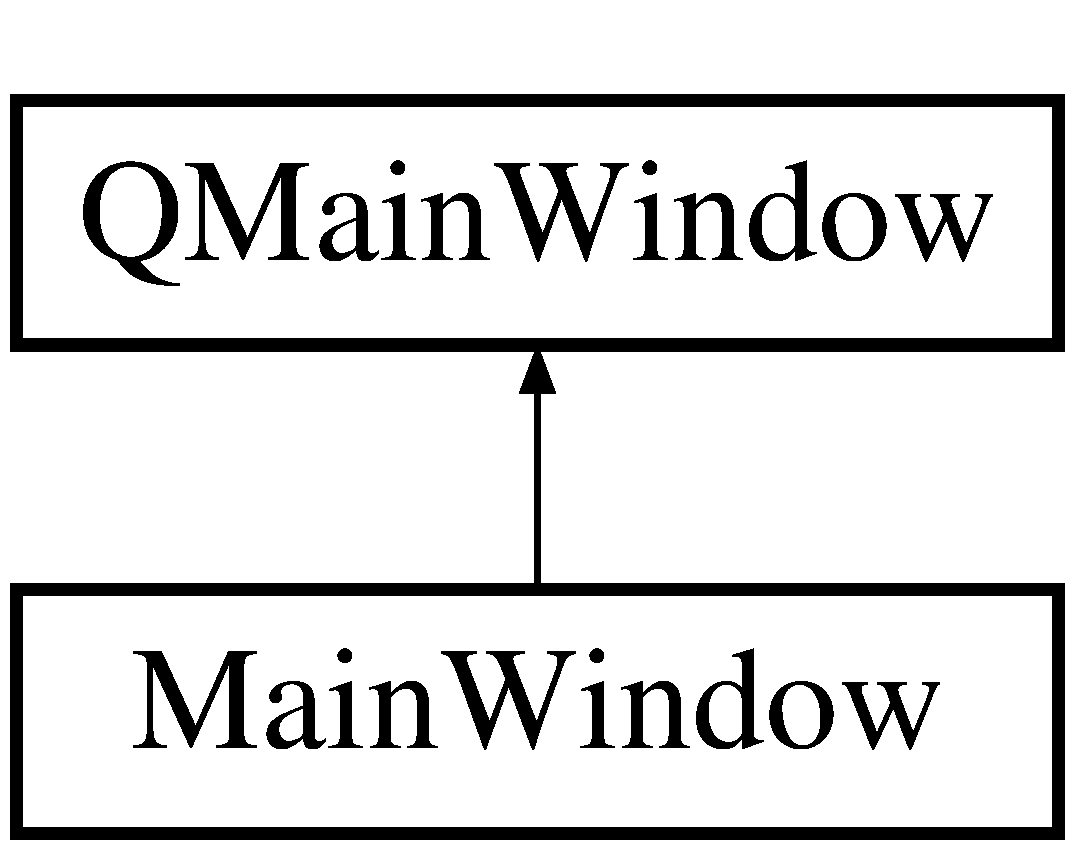
\includegraphics[height=2.000000cm]{classMainWindow}
\end{center}
\end{figure}
\subsection*{Public Member Functions}
\begin{DoxyCompactItemize}
\item 
\hyperlink{classMainWindow_a8b244be8b7b7db1b08de2a2acb9409db}{Main\+Window} (Q\+Widget $\ast$parent=0)
\item 
\hyperlink{classMainWindow_ae98d00a93bc118200eeef9f9bba1dba7}{$\sim$\+Main\+Window} ()
\item 
void \hyperlink{classMainWindow_a7c2ac5ce98b2a5de2928e730e48dcfd0}{Abrir\+Dialog} ()
\item 
void \hyperlink{classMainWindow_aa878ce12d90414ed30463be34b4eea91}{Plotar} ()
\end{DoxyCompactItemize}


\subsection{Detailed Description}
Classe que a interação com a segunda tela da interface grafica. 

\subsection{Constructor \& Destructor Documentation}
\hypertarget{classMainWindow_a8b244be8b7b7db1b08de2a2acb9409db}{}\index{Main\+Window@{Main\+Window}!Main\+Window@{Main\+Window}}
\index{Main\+Window@{Main\+Window}!Main\+Window@{Main\+Window}}
\subsubsection[{Main\+Window}]{\setlength{\rightskip}{0pt plus 5cm}Main\+Window\+::\+Main\+Window (
\begin{DoxyParamCaption}
\item[{Q\+Widget $\ast$}]{parent = {\ttfamily 0}}
\end{DoxyParamCaption}
)\hspace{0.3cm}{\ttfamily [explicit]}}\label{classMainWindow_a8b244be8b7b7db1b08de2a2acb9409db}
Construtor padrão da classe 
\begin{DoxyParams}{Parameters}
{\em parent} & \\
\hline
\end{DoxyParams}
\hypertarget{classMainWindow_ae98d00a93bc118200eeef9f9bba1dba7}{}\index{Main\+Window@{Main\+Window}!````~Main\+Window@{$\sim$\+Main\+Window}}
\index{````~Main\+Window@{$\sim$\+Main\+Window}!Main\+Window@{Main\+Window}}
\subsubsection[{$\sim$\+Main\+Window}]{\setlength{\rightskip}{0pt plus 5cm}Main\+Window\+::$\sim$\+Main\+Window (
\begin{DoxyParamCaption}
{}
\end{DoxyParamCaption}
)}\label{classMainWindow_ae98d00a93bc118200eeef9f9bba1dba7}
Destrutor padrão 

\subsection{Member Function Documentation}
\hypertarget{classMainWindow_a7c2ac5ce98b2a5de2928e730e48dcfd0}{}\index{Main\+Window@{Main\+Window}!Abrir\+Dialog@{Abrir\+Dialog}}
\index{Abrir\+Dialog@{Abrir\+Dialog}!Main\+Window@{Main\+Window}}
\subsubsection[{Abrir\+Dialog}]{\setlength{\rightskip}{0pt plus 5cm}void Main\+Window\+::\+Abrir\+Dialog (
\begin{DoxyParamCaption}
{}
\end{DoxyParamCaption}
)}\label{classMainWindow_a7c2ac5ce98b2a5de2928e730e48dcfd0}
Abre a primeira tela do sistema, que configura o sistema \hypertarget{classMainWindow_aa878ce12d90414ed30463be34b4eea91}{}\index{Main\+Window@{Main\+Window}!Plotar@{Plotar}}
\index{Plotar@{Plotar}!Main\+Window@{Main\+Window}}
\subsubsection[{Plotar}]{\setlength{\rightskip}{0pt plus 5cm}void Main\+Window\+::\+Plotar (
\begin{DoxyParamCaption}
{}
\end{DoxyParamCaption}
)}\label{classMainWindow_aa878ce12d90414ed30463be34b4eea91}
Plota o grafico da cluster do H\+D 

The documentation for this class was generated from the following files\+:\begin{DoxyCompactItemize}
\item 
Gerenciador\+De\+Disco/mainwindow.\+h\item 
Gerenciador\+De\+Disco/mainwindow.\+cpp\end{DoxyCompactItemize}

\hypertarget{classUi_1_1MainWindow}{}\section{Ui\+:\+:Main\+Window Class Reference}
\label{classUi_1_1MainWindow}\index{Ui\+::\+Main\+Window@{Ui\+::\+Main\+Window}}
Inheritance diagram for Ui\+:\+:Main\+Window\+:\begin{figure}[H]
\begin{center}
\leavevmode
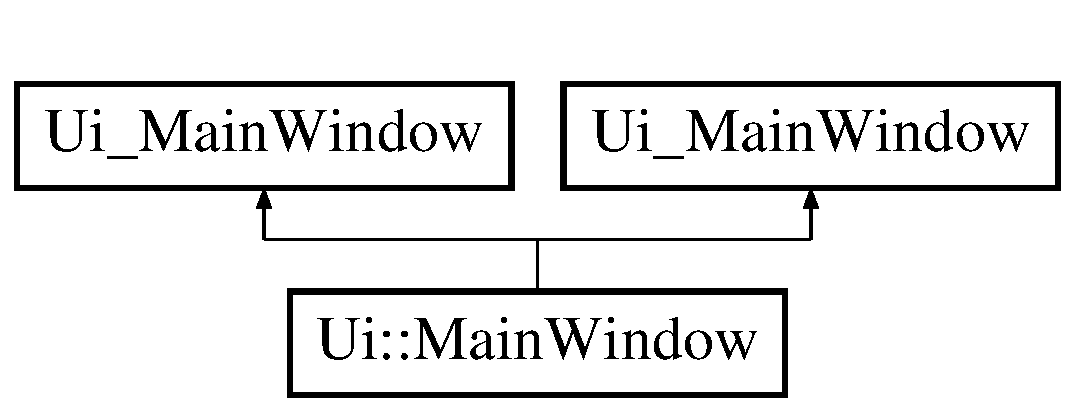
\includegraphics[height=2.000000cm]{classUi_1_1MainWindow}
\end{center}
\end{figure}
\subsection*{Additional Inherited Members}


The documentation for this class was generated from the following file\+:\begin{DoxyCompactItemize}
\item 
build-\/\+Gerenciador\+De\+Disco-\/\+Desktop\+\_\+\+Qt\+\_\+5\+\_\+4\+\_\+1\+\_\+\+G\+C\+C\+\_\+64bit-\/\+Debug/ui\+\_\+mainwindow.\+h\end{DoxyCompactItemize}

\hypertarget{structLista_1_1node}{}\section{Lista$<$ type $>$\+:\+:node Struct Reference}
\label{structLista_1_1node}\index{Lista$<$ type $>$\+::node@{Lista$<$ type $>$\+::node}}


{\ttfamily \#include $<$lista.\+h$>$}

\subsection*{Public Attributes}
\begin{DoxyCompactItemize}
\item 
type \hyperlink{structLista_1_1node_a296293814eb82b9a0ff188a8a4c7aedc}{val}
\item 
\hyperlink{structLista_1_1node}{node} $\ast$ \hyperlink{structLista_1_1node_a352a7913205b61620f95559234ebbf40}{next} = N\+U\+L\+L
\end{DoxyCompactItemize}


\subsection{Detailed Description}
\subsubsection*{template$<$class type$>$struct Lista$<$ type $>$\+::node}

Estrutura de um nó da lista 

\subsection{Member Data Documentation}
\hypertarget{structLista_1_1node_a352a7913205b61620f95559234ebbf40}{}\index{Lista\+::node@{Lista\+::node}!next@{next}}
\index{next@{next}!Lista\+::node@{Lista\+::node}}
\subsubsection[{next}]{\setlength{\rightskip}{0pt plus 5cm}template$<$class type$>$ {\bf node}$\ast$ {\bf Lista}$<$ type $>$\+::node\+::next = N\+U\+L\+L}\label{structLista_1_1node_a352a7913205b61620f95559234ebbf40}
Armazena o endereço de memória para o próximo nó. Por padrão é N\+U\+L\+O \hypertarget{structLista_1_1node_a296293814eb82b9a0ff188a8a4c7aedc}{}\index{Lista\+::node@{Lista\+::node}!val@{val}}
\index{val@{val}!Lista\+::node@{Lista\+::node}}
\subsubsection[{val}]{\setlength{\rightskip}{0pt plus 5cm}template$<$class type$>$ type {\bf Lista}$<$ type $>$\+::node\+::val}\label{structLista_1_1node_a296293814eb82b9a0ff188a8a4c7aedc}
Armazena o valor do nó atual 

The documentation for this struct was generated from the following file\+:\begin{DoxyCompactItemize}
\item 
Gerenciador\+De\+Disco/lista.\+h\end{DoxyCompactItemize}

\hypertarget{structqt__meta__stringdata__Dialog__t}{\section{qt\+\_\+meta\+\_\+stringdata\+\_\+\+Dialog\+\_\+t Struct Reference}
\label{structqt__meta__stringdata__Dialog__t}\index{qt\+\_\+meta\+\_\+stringdata\+\_\+\+Dialog\+\_\+t@{qt\+\_\+meta\+\_\+stringdata\+\_\+\+Dialog\+\_\+t}}
}
\subsection*{Public Attributes}
\begin{DoxyCompactItemize}
\item 
\hypertarget{structqt__meta__stringdata__Dialog__t_ae8df3bc8b623c73ab4d9b75541fe0ed8}{Q\+Byte\+Array\+Data {\bfseries data} \mbox{[}5\mbox{]}}\label{structqt__meta__stringdata__Dialog__t_ae8df3bc8b623c73ab4d9b75541fe0ed8}

\item 
\hypertarget{structqt__meta__stringdata__Dialog__t_aa3d88739476830b302bbe2887068499e}{char {\bfseries stringdata} \mbox{[}71\mbox{]}}\label{structqt__meta__stringdata__Dialog__t_aa3d88739476830b302bbe2887068499e}

\end{DoxyCompactItemize}


The documentation for this struct was generated from the following file\+:\begin{DoxyCompactItemize}
\item 
Gerenciador\+De\+Disco/moc\+\_\+dialog.\+cpp\end{DoxyCompactItemize}

\hypertarget{structqt__meta__stringdata__MainWindow__t}{\section{qt\+\_\+meta\+\_\+stringdata\+\_\+\+Main\+Window\+\_\+t Struct Reference}
\label{structqt__meta__stringdata__MainWindow__t}\index{qt\+\_\+meta\+\_\+stringdata\+\_\+\+Main\+Window\+\_\+t@{qt\+\_\+meta\+\_\+stringdata\+\_\+\+Main\+Window\+\_\+t}}
}
\subsection*{Public Attributes}
\begin{DoxyCompactItemize}
\item 
\hypertarget{structqt__meta__stringdata__MainWindow__t_ae8888f3a82b4bd7597ba5dad592aeec6}{Q\+Byte\+Array\+Data {\bfseries data} \mbox{[}8\mbox{]}}\label{structqt__meta__stringdata__MainWindow__t_ae8888f3a82b4bd7597ba5dad592aeec6}

\item 
\hypertarget{structqt__meta__stringdata__MainWindow__t_a36f09c6ee58fefb768d55e0f8051d219}{char {\bfseries stringdata} \mbox{[}130\mbox{]}}\label{structqt__meta__stringdata__MainWindow__t_a36f09c6ee58fefb768d55e0f8051d219}

\end{DoxyCompactItemize}


The documentation for this struct was generated from the following file\+:\begin{DoxyCompactItemize}
\item 
Gerenciador\+De\+Disco/moc\+\_\+mainwindow.\+cpp\end{DoxyCompactItemize}

\hypertarget{classSetor}{}\section{Setor Class Reference}
\label{classSetor}\index{Setor@{Setor}}
\subsection*{Public Member Functions}
\begin{DoxyCompactItemize}
\item 
\hypertarget{classSetor_ad547a9f194a2cb2d763371f16c42e99e}{}{\bfseries Setor} (int id)\label{classSetor_ad547a9f194a2cb2d763371f16c42e99e}

\item 
\hypertarget{classSetor_a5ab13049bf55eddc4586212567a936ed}{}{\bfseries Setor} (int id, int inicio, int fim)\label{classSetor_a5ab13049bf55eddc4586212567a936ed}

\item 
\hypertarget{classSetor_ae31a039bd0ac2d1c76802198abf8f076}{}int {\bfseries get\+Inicio} ()\label{classSetor_ae31a039bd0ac2d1c76802198abf8f076}

\item 
\hypertarget{classSetor_a5f46674630604f4ef6215985bbc97a9e}{}int {\bfseries get\+Fim} ()\label{classSetor_a5f46674630604f4ef6215985bbc97a9e}

\item 
\hypertarget{classSetor_a3a86ea9d1832d230fb7abe4fafbe0bf5}{}int {\bfseries get\+Id} ()\label{classSetor_a3a86ea9d1832d230fb7abe4fafbe0bf5}

\end{DoxyCompactItemize}


The documentation for this class was generated from the following files\+:\begin{DoxyCompactItemize}
\item 
Gerenciador\+De\+Disco/setor.\+h\item 
Gerenciador\+De\+Disco/setor.\+cpp\end{DoxyCompactItemize}

\hypertarget{classUi__Dialog}{}\section{Ui\+\_\+\+Dialog Class Reference}
\label{classUi__Dialog}\index{Ui\+\_\+\+Dialog@{Ui\+\_\+\+Dialog}}
Inheritance diagram for Ui\+\_\+\+Dialog\+:\begin{figure}[H]
\begin{center}
\leavevmode
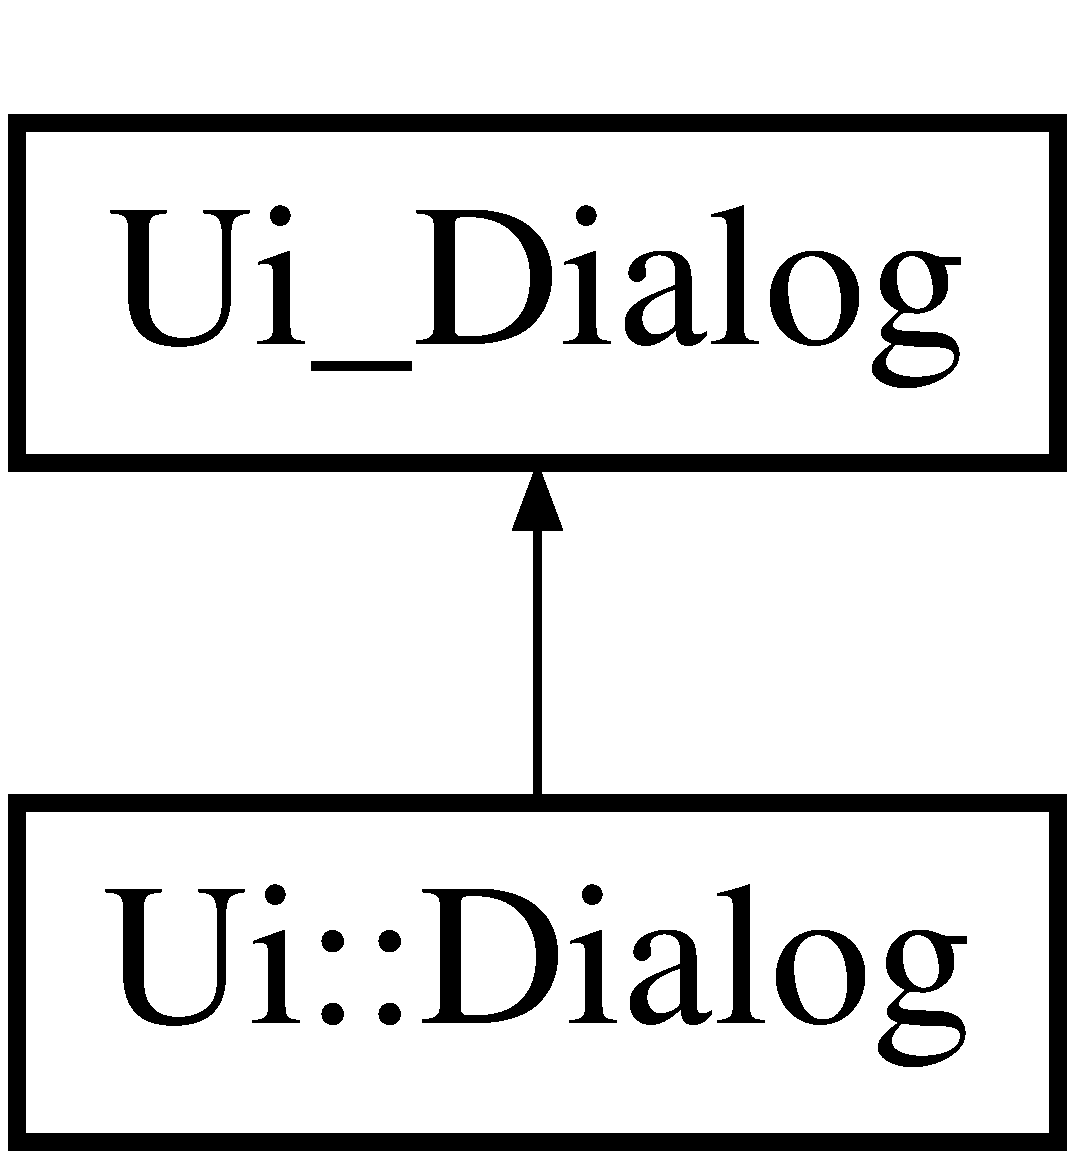
\includegraphics[height=2.000000cm]{classUi__Dialog}
\end{center}
\end{figure}
\subsection*{Public Member Functions}
\begin{DoxyCompactItemize}
\item 
\hypertarget{classUi__Dialog_a4f6a478c3ecdafabffb17b39cb26444a}{}void {\bfseries setup\+Ui} (Q\+Dialog $\ast$\hyperlink{classDialog}{Dialog})\label{classUi__Dialog_a4f6a478c3ecdafabffb17b39cb26444a}

\item 
\hypertarget{classUi__Dialog_afa0ccb6f716ca6178260522a193c250e}{}void {\bfseries retranslate\+Ui} (Q\+Dialog $\ast$\hyperlink{classDialog}{Dialog})\label{classUi__Dialog_afa0ccb6f716ca6178260522a193c250e}

\item 
\hypertarget{classUi__Dialog_a4f6a478c3ecdafabffb17b39cb26444a}{}void {\bfseries setup\+Ui} (Q\+Dialog $\ast$\hyperlink{classDialog}{Dialog})\label{classUi__Dialog_a4f6a478c3ecdafabffb17b39cb26444a}

\item 
\hypertarget{classUi__Dialog_afa0ccb6f716ca6178260522a193c250e}{}void {\bfseries retranslate\+Ui} (Q\+Dialog $\ast$\hyperlink{classDialog}{Dialog})\label{classUi__Dialog_afa0ccb6f716ca6178260522a193c250e}

\end{DoxyCompactItemize}
\subsection*{Public Attributes}
\begin{DoxyCompactItemize}
\item 
\hypertarget{classUi__Dialog_a5991d63e5d8f30a9a29671aeb370439a}{}Q\+Dialog\+Button\+Box $\ast$ {\bfseries button\+Box}\label{classUi__Dialog_a5991d63e5d8f30a9a29671aeb370439a}

\item 
\hypertarget{classUi__Dialog_a7f0bb3c686eebfcee9c7a439fc1fe79c}{}Q\+Label $\ast$ {\bfseries label}\label{classUi__Dialog_a7f0bb3c686eebfcee9c7a439fc1fe79c}

\item 
\hypertarget{classUi__Dialog_a6d519cb52632a0216fef7bb9a429af41}{}Q\+Widget $\ast$ {\bfseries layout\+Widget}\label{classUi__Dialog_a6d519cb52632a0216fef7bb9a429af41}

\item 
\hypertarget{classUi__Dialog_a5218e699bf6de0048f2fbe5fa03a34de}{}Q\+Form\+Layout $\ast$ {\bfseries form\+Layout}\label{classUi__Dialog_a5218e699bf6de0048f2fbe5fa03a34de}

\item 
\hypertarget{classUi__Dialog_a6f921061e303332855576b1d2b9852f7}{}Q\+Label $\ast$ {\bfseries quant\+Setor}\label{classUi__Dialog_a6f921061e303332855576b1d2b9852f7}

\item 
\hypertarget{classUi__Dialog_ae1c6f4f8e9a96b614f070f3e43840c38}{}Q\+Spin\+Box $\ast$ {\bfseries val\+Quant\+Setor}\label{classUi__Dialog_ae1c6f4f8e9a96b614f070f3e43840c38}

\item 
\hypertarget{classUi__Dialog_ae605b68db90d62dbb12a846beade4880}{}Q\+Label $\ast$ {\bfseries tam\+Setor}\label{classUi__Dialog_ae605b68db90d62dbb12a846beade4880}

\item 
\hypertarget{classUi__Dialog_a2ca544457e671fea81b6656eb75a9142}{}Q\+Spin\+Box $\ast$ {\bfseries val\+Tam\+Setor}\label{classUi__Dialog_a2ca544457e671fea81b6656eb75a9142}

\item 
\hypertarget{classUi__Dialog_a457a5e3a5d2faf1fb56a5a231dca1ce4}{}Q\+Label $\ast$ {\bfseries tam\+Disco}\label{classUi__Dialog_a457a5e3a5d2faf1fb56a5a231dca1ce4}

\item 
\hypertarget{classUi__Dialog_afd9ae775d0784ce5089010610594a598}{}Q\+Label $\ast$ {\bfseries val\+Tam\+Disco}\label{classUi__Dialog_afd9ae775d0784ce5089010610594a598}

\end{DoxyCompactItemize}


The documentation for this class was generated from the following file\+:\begin{DoxyCompactItemize}
\item 
build-\/\+Gerenciador\+De\+Disco-\/\+Desktop\+\_\+\+Qt\+\_\+5\+\_\+4\+\_\+1\+\_\+\+G\+C\+C\+\_\+64bit-\/\+Debug/ui\+\_\+dialog.\+h\end{DoxyCompactItemize}

\hypertarget{classUi__MainWindow}{}\section{Ui\+\_\+\+Main\+Window Class Reference}
\label{classUi__MainWindow}\index{Ui\+\_\+\+Main\+Window@{Ui\+\_\+\+Main\+Window}}
Inheritance diagram for Ui\+\_\+\+Main\+Window\+:\begin{figure}[H]
\begin{center}
\leavevmode
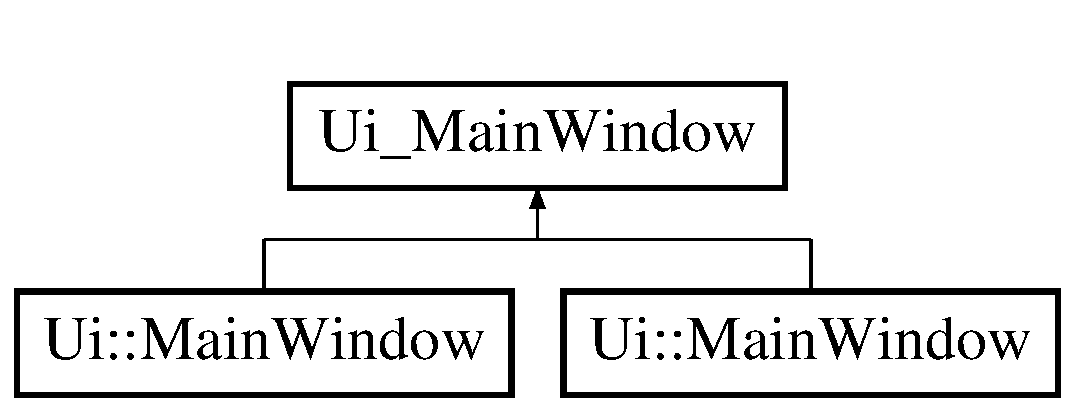
\includegraphics[height=2.000000cm]{classUi__MainWindow}
\end{center}
\end{figure}
\subsection*{Public Member Functions}
\begin{DoxyCompactItemize}
\item 
\hypertarget{classUi__MainWindow_acf4a0872c4c77d8f43a2ec66ed849b58}{}void {\bfseries setup\+Ui} (Q\+Main\+Window $\ast$\hyperlink{classMainWindow}{Main\+Window})\label{classUi__MainWindow_acf4a0872c4c77d8f43a2ec66ed849b58}

\item 
\hypertarget{classUi__MainWindow_a097dd160c3534a204904cb374412c618}{}void {\bfseries retranslate\+Ui} (Q\+Main\+Window $\ast$\hyperlink{classMainWindow}{Main\+Window})\label{classUi__MainWindow_a097dd160c3534a204904cb374412c618}

\item 
\hypertarget{classUi__MainWindow_acf4a0872c4c77d8f43a2ec66ed849b58}{}void {\bfseries setup\+Ui} (Q\+Main\+Window $\ast$\hyperlink{classMainWindow}{Main\+Window})\label{classUi__MainWindow_acf4a0872c4c77d8f43a2ec66ed849b58}

\item 
\hypertarget{classUi__MainWindow_a097dd160c3534a204904cb374412c618}{}void {\bfseries retranslate\+Ui} (Q\+Main\+Window $\ast$\hyperlink{classMainWindow}{Main\+Window})\label{classUi__MainWindow_a097dd160c3534a204904cb374412c618}

\end{DoxyCompactItemize}
\subsection*{Public Attributes}
\begin{DoxyCompactItemize}
\item 
\hypertarget{classUi__MainWindow_a6600dd3bdd3d55e535659e4a4096ea48}{}Q\+Widget $\ast$ {\bfseries central\+Widget}\label{classUi__MainWindow_a6600dd3bdd3d55e535659e4a4096ea48}

\item 
\hypertarget{classUi__MainWindow_a6356443dc067ef5164e2f4dc834e640b}{}Q\+Widget $\ast$ {\bfseries layout\+Widget}\label{classUi__MainWindow_a6356443dc067ef5164e2f4dc834e640b}

\item 
\hypertarget{classUi__MainWindow_ac4586abe48f0aabf940b0dc2df3772ed}{}Q\+Grid\+Layout $\ast$ {\bfseries grid\+Layout}\label{classUi__MainWindow_ac4586abe48f0aabf940b0dc2df3772ed}

\item 
\hypertarget{classUi__MainWindow_aed1f878fc5d696cd850df6f1777f29f8}{}Q\+Label $\ast$ {\bfseries Label\+Nome}\label{classUi__MainWindow_aed1f878fc5d696cd850df6f1777f29f8}

\item 
\hypertarget{classUi__MainWindow_a4e625071b6eb57c1ab2bce6141469044}{}Q\+Line\+Edit $\ast$ {\bfseries Campo\+Nome}\label{classUi__MainWindow_a4e625071b6eb57c1ab2bce6141469044}

\item 
\hypertarget{classUi__MainWindow_a5daf68cc652b2f712d02806bab4bf81a}{}Q\+Push\+Button $\ast$ {\bfseries excluir}\label{classUi__MainWindow_a5daf68cc652b2f712d02806bab4bf81a}

\item 
\hypertarget{classUi__MainWindow_a610e58a1a3a371cd68fb5db0b154d8d3}{}Q\+Push\+Button $\ast$ {\bfseries desfragmentar}\label{classUi__MainWindow_a610e58a1a3a371cd68fb5db0b154d8d3}

\item 
\hypertarget{classUi__MainWindow_a73489a4788a12478496973453b856d24}{}Q\+Label $\ast$ {\bfseries Label\+Valor}\label{classUi__MainWindow_a73489a4788a12478496973453b856d24}

\item 
\hypertarget{classUi__MainWindow_ac65a7a5295819f72eed23a44569f92f5}{}Q\+Line\+Edit $\ast$ {\bfseries Campo\+Valor}\label{classUi__MainWindow_ac65a7a5295819f72eed23a44569f92f5}

\item 
\hypertarget{classUi__MainWindow_a923071e00862edfd4b7dae1acfa2ce72}{}Q\+Push\+Button $\ast$ {\bfseries salvar}\label{classUi__MainWindow_a923071e00862edfd4b7dae1acfa2ce72}

\item 
\hypertarget{classUi__MainWindow_a1a6dc24545f27bd86e948aea1f968336}{}Q\+Push\+Button $\ast$ {\bfseries listar}\label{classUi__MainWindow_a1a6dc24545f27bd86e948aea1f968336}

\item 
\hypertarget{classUi__MainWindow_ab5edaf931c456221366ab8b2680a983e}{}Q\+Push\+Button $\ast$ {\bfseries formatar}\label{classUi__MainWindow_ab5edaf931c456221366ab8b2680a983e}

\item 
\hypertarget{classUi__MainWindow_a1597346a152c37a0fcd697db06771a0a}{}Q\+Push\+Button $\ast$ {\bfseries buscar}\label{classUi__MainWindow_a1597346a152c37a0fcd697db06771a0a}

\item 
\hypertarget{classUi__MainWindow_afd6631fbb0b169e83b16f1ac59d65ad5}{}Q\+Text\+Browser $\ast$ {\bfseries grafico}\label{classUi__MainWindow_afd6631fbb0b169e83b16f1ac59d65ad5}

\item 
\hypertarget{classUi__MainWindow_a98cd045ec752a28ac23816806cceb982}{}Q\+Text\+Browser $\ast$ {\bfseries lista}\label{classUi__MainWindow_a98cd045ec752a28ac23816806cceb982}

\item 
\hypertarget{classUi__MainWindow_a502a50d7dc22415f511336bdfb4318b9}{}Q\+Menu\+Bar $\ast$ {\bfseries menu\+Bar}\label{classUi__MainWindow_a502a50d7dc22415f511336bdfb4318b9}

\item 
\hypertarget{classUi__MainWindow_abca26371605d7c5235fab5188d4bdcf7}{}Q\+Tool\+Bar $\ast$ {\bfseries main\+Tool\+Bar}\label{classUi__MainWindow_abca26371605d7c5235fab5188d4bdcf7}

\item 
\hypertarget{classUi__MainWindow_afa919f3af6f2f526a70f1fa331f63724}{}Q\+Status\+Bar $\ast$ {\bfseries status\+Bar}\label{classUi__MainWindow_afa919f3af6f2f526a70f1fa331f63724}

\end{DoxyCompactItemize}


The documentation for this class was generated from the following file\+:\begin{DoxyCompactItemize}
\item 
build-\/\+Gerenciador\+De\+Disco-\/\+Desktop\+\_\+\+Qt\+\_\+5\+\_\+4\+\_\+1\+\_\+\+G\+C\+C\+\_\+64bit-\/\+Debug/ui\+\_\+mainwindow.\+h\end{DoxyCompactItemize}

%--- End generated contents ---

% Index
\backmatter
\newpage
\phantomsection
\clearemptydoublepage
\addcontentsline{toc}{chapter}{Index}
\printindex

\end{document}
